\chapter{Voronoi-Basierter Multi-Minimax Algorithmus}
\label{cha:voronoi}

In diesem Kapitel stellen wir den Multi-Minimax-Algorithmus und eine auf Voronoi-Diagrammen basierende Situationsbewertung vor. Zudem beschreiben wir zusätzliche Erweiterungen, die den Algorithmus bestmöglich auf Spe\_ed anpassen.

\section{Multi-Minimax}

Es existieren bereits mehrere Ansätze um Minimax auf Multiplayer-Spiele zu erweitern: \textit{Paranoid \cite{Sturtevant.2006}, Max\textsuperscript{n} \cite{.1986}}, \textit{Best Reply Search} \cite{Schadd.2011} und Multi-Minimax \cite{Perez.2019}. Multi-Minimax wurde in der Arbeit von Perez und Oommen gegen die oben genannten Algorithmen am Spiel \textit{Light Cycles} getestet. Der vorgestellte Algorithmus erzielte dabei sowohl bei 4-Spieler-Situationen als auch bei 6-Spieler-Situatioen bei über 20.000 getesteten Spielen die besten Ergebnisse. Darüber hinaus bietet er uns den Vorteil, dass er bereits für simultane Spiele, also Spiele mit gleichzeitigen Zügen ausgelegt ist. Der Algorithmus läuft in \textit{O(nb\textsuperscript{d})} für n = Spieleranzahl, b = \textit{branchingfactor}\footnote{Anzahl der Aktionen} und d = Anzahl der Spielrunden \cite{Perez.2019}. Daher verwenden wir Multi-Minimax auch für unseren Lösungsansatz.

Beim Multi-Minimax-Algorithmus tritt der maximierende Spieler immer isoliert gegen einen minimierenden Spieler an. Nachdem jeder Gegenspieler isoliert betrachtet wurde, wird die eigene Aktion basierend auf dem besten Gegenspieler gewählt. Dabei verwendet der Algorithmus Alpha-Beta Pruning und die in Kapitel \ref{cha:spieltheorie} beschriebene Minimax-Routine. In Abbildung \ref{fig:multiminimax} ist ein Entscheidungsbaum der Tiefe drei abgebildet.

Die Heuristik die Perez und Oommen für die Situationsbewertung verwenden, ist simpel. Falls der Gegenspieler nicht mehr aktiv ist und der eigene Spieler noch mögliche Züge hat, die nicht zum Tod führen, wird die Situation mit dem best-möglichen Wert unendlich bewertet. Andernfalls wird die Situation mit der erreichten Suchtiefe bewertet. Diese Heuristik ist sehr praktisch für kleine Spielfelder (12x12 im Fall von Perez und Oommen), da sie wenig Rechenaufwand benötigt und somit fast alle möglichen Züge berechnet werden können. In unserem Fall ist sie aber nicht ideal, weil das Spielfeld bei Spe\_ed bis 80x80 groß werden kann. Dafür ist eine Heuristik notwendig, die Informationen über das ganze Spielfeld liefert und einschätzt, wie gut ein Spieler momentan ist - unabhängig davon, ob er in x Zügen sterben würde. Deshalb haben wir die in Kapitel \ref{cha:voronoi} vorgestellte Voronoi-Heuristik gewählt.

\begin{figure}[ht]
    \centering
    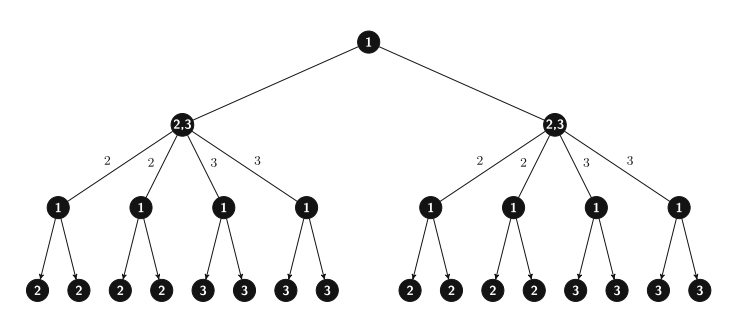
\includegraphics[width=1\textwidth]{img/multiminimax.PNG}
    \caption[Multi-Minimax]{Multi-Minimax Repräsentation für 3 Spieler und branching-Faktor 2. Die Knoten geben an, welcher Spieler als nächstes an der Reihe ist, die Kanten repräsentieren die Aktionen. Grafik aus \textit{Multi-Minimax: A New AI Paradigm for Simultaneously-Played Multi-player Games \cite{Perez.2019}}}
	\label{fig:multiminimax}
\end{figure}

\section{Voronoi-Heuristik}
\label{cha:voronoi_sec}

Ein Voronoi-Diagramm (vgl. Abbildung \ref{fig:voronoi}) gibt an, welche Felder des Spielfeldes von welchem Spieler zuerst erreicht werden können. Felder die gleichzeitig erreicht werden können werden als \textit{battlefront} bezeichnet (Lila Felder in Abbildung \ref{fig:voronoi}). Die Idee zu diesem Ansatz kam erstmals während der \textit{Google AI Challenge}\footnote{https://de.wikipedia.org/wiki/AI Challenge} auf \cite{AndySloane.2010}. Die Voronoi-Heuristik bewertet nun eine Spielsituation basierend auf der Differenz der zuerst erreichbaren Felder des eigenen Agenten und des jeweiligen Min-Agenten. Da wir bei Spe\_ed im Gegensatz zur \textit{Google AI Challenge} verschiedene Geschwindigkeiten haben, müssten wir das Voronoi-Diagramm unter Betrachtung der derzeitigen Geschwindigkeiten und möglicher Geschwindigkeitsänderungen aller Spieler berechnen. Wir haben diese Erweiterung implementiert und evaluiert, sind aber zu dem Schluss gekommen, dass der gewonnene Vorteil im Vergleich zum stark erhöhten Rechenaufwand zu gering ist. Eine Erweiterung und Verbesserung der Voronoi-Heuristik für das klassische \textit{Tron}-Game ist die \textit{Tree-of-Chambers}-Heuristik \cite{AndySloane.2010, Kang.2012}. Diese ist jedoch für Spielfelder mit vielen einzelnen Lücken ungeeignet \cite{Kang.2012}. Da bei Spe\_ed ein zerklüftetes Spielfeld durch das regelmäßige Entstehen von Lücken häufiger vorkommt, haben wir uns schlussendlich für die Voronoi-Heuristik ohne Tree-of-Chambers-Erweiterung entschieden.

\begin{figure}[ht]
    \centering
    \includegraphics[width=0.4\textwidth]{img/voronoi.PNG}
    \caption[Voronoi-Diagramm]{Voronoi-Diagramm für vier Spieler auf einem 50x50 Feld. Spielerpositionen in Schwarz dargestellt; Voronoi-Regionen der jeweiligen Spieler in Grün, Rot, Gelb und Türkis; Battlefronts in Lila.}
	\label{fig:voronoi}
\end{figure}

\section{Erweiterungen}
\label{cha:Erweiterungen}

Die beiden vorgestellten Grundkonzepte \textit{Multi-Minimax} und \textit{Voronoi-Heuristik} haben wir durch einige Erweiterungen angepasst, um sie bestmöglich für Spe\_ed verwenden zu können. Diese Erweiterungen werden im Folgenden vorgestellt.

\subsection{Vorsortierung der Aktionen}

Beim Alpha-Beta-Pruning können mehr Pfade eliminiert werden, wenn die Aktionen für die Mulit-Minimax-Suche nach ihrer Ausführungswahrscheinlichkeit vorsortiert werden. Durch Beobachtungen hat sich folgende Reihenfolge als optimal ergeben:
\begin{enumerate}
    \item change\_nothing
    \item turn\_left
    \item turn\_right
    \item speed\_up
    \item slow\_down
\end{enumerate}

\subsection{Endgame-Erkennung}

Wir überprüfen zu Beginn des Algorithmus ob wir uns in einem \textit{Endgame} befinden. Wir befinden uns in einem \textit{Endgame}, sobald wir keinen Gegner mehr direkt erreichen können, ohne dabei über eine Mauer zu springen. Ein Endgame wird wieder aufgelöst, sobald wir in den Bereich eines Gegners springen oder ein Gegner in unseren Bereich springt. Sobald wir uns in einem Endgame befinden, simulieren wir nur die eigenen Züge und ignorieren das Verhalten der Gegner. Dies erlaubt uns, eine größere Tiefe für den Multi-Minimax Algorithmus zu erreichen und somit in einer gewinnenden Position unseren verfügbaren Bereich nahezu perfekt auszufüllen und in einer verlierenden Position mehr Möglichkeiten zu evaluieren, um aus unserem Bereich heraus zuspringen und somit das Endgame aufzulösen.  

\subsection{Wall-Hugging}

Wir fügen, wie es Andy Sloane in \cite{AndySloane.2010} beschreibt, einen \textit{territory-bonus} hinzu. Dabei werden offene Felder aus der eigenen Voronoi-Region höher gewichtet als Felder mit mehr Wänden. Dies führt automatisch dazu, das unser Agent im Falle eines Voronoi-Gleichstands eher an Wänden entlang fährt und somit seinen eigenen Platz weniger verbaut. 

\subsection{Reduktion der betrachteten Gegner}

Da bei sechs Spielern der Berechnungsaufwand für Multi-Minimax im Vergleich zu weniger Spielern stark erhöht ist, schränken wir die betrachteten Gegenspieler ein. Wir ermitteln gleichzeitig zur Endgame Erkennung die Gegenspieler, deren Voronoi-Regionen auf unsere treffen. Wir schließen Gegenspieler aus, die wir nicht erreichen können, weil sie eine Wand von uns trennt oder ein weiterer Spieler dazwischen positioniert ist. Wir gehen davon aus, dass das Verhalten dieser Spieler für uns vorerst nicht relevant ist. Wären wir zum Beispiel in Abbildung \ref{fig:voronoi} der Spieler mit der grünen Voronoi-Region, würden wir den Spieler mit der gelben Voronoi-Region vorerst nicht betrachten, da diese Voronoi-Regionen nicht aufeinandertreffen.

\subsection{Einschränkung der eigenen Geschwindigkeit}

Wir haben beobachtet, dass unser Agent bei höheren Geschwindigkeiten teilweise schlechte Entscheidungen trifft. Die Suchtiefe, die wir im Falle von knappen \textit{Deadlines} (unter 8 Sekunden) erreichen, reicht nicht aus, um bei hohen Geschwindigkeiten Kollisionen zu vermeiden. Deshalb haben wir uns entschieden, die maximale Geschwindigkeit unseres Agenten auf drei zu beschränken. Diese Geschwindigkeit ermöglicht es uns trotzdem noch die regelmäßig entstehende Lücke geschickt zu nutzen. Wir heben diese Einschränkung auf, sobald wir uns im Endgame befinden. Dadurch kann unser Agent mehr Möglichkeiten berechnen, im Falle eines verlierenden Endgames aus dem eigenen Bereich zu springen und eine verlierende Position zu einer gewinnenden zu drehen. 

\subsection{\acrlong{DFID}}

Für die Berechnung der nächsten Aktion wird in Spe\_ed jeweils eine Zugzeit vorgegeben. Somit müssten wir bei der Tiefensuche die maximale Tiefe für den Suchbaum genau so wählen, dass alle Äste in der vorgegebenen Zeit abgearbeitet werden. Dies ist offensichtlich sehr fehleranfällig. Wählen wir hingegen einen Breitensuche-Ansatz, wird schnell viel Speicherplatz benötigt. Einen Kompromiss zwischen beiden Varianten bietet \acrfull{DFID}. Dabei wird die Tiefensuche auf eine maximale Tiefe begrenzt, sobald diese Tiefe abgeschlossen ist, wird die maximale Tiefe erhöht und der Baum erneut durchlaufen. Das verursacht zwar, dass die oberen Bereiche des Baumes (unnötig) mehrfach berechnet werden, da der Baum nach unten allerdings exponentiell größer wird, ist dies verschmerzbar. \cite{Korf.1985}

Somit wird die gewählte Aktion mit steigender Suchtiefe inkrementell verbessert. Zum einen garantieren wir damit, dass unser Algorithmus auch bei kurzen Zugzeiten eine passende Aktion findet. Zum anderen nutzt der Algorithmus die volle Zugzeit aus und sucht bei längeren Zeiten nach Lösungen in tieferen Suchebenen. Wir starten die Berechnung der auszuführenden Aktion in einem Subprozess, während im Hauptprozess die aktuelle Serverzeit abgefragt und die verfügbare Zeit berechnet wird. Sobald die Zeit abgelaufen ist, terminiert der Hauptprozess das \acrshort{DFID} und erhält über eine zwischen den Prozessen geteilte Variable die auszuführende Aktion. Zur Kommunikation mit dem Server verwenden wir Python's \textit{asyncio}\footnote{https://docs.python.org/3/library/asyncio.html}.


\subsection{Multiprocessing}
Zur Verbesserung der Berechnungsgeschwindigkeit wird \textit{Multiprocessing} verwendet. Dabei wird die \acrshort{DFID} Methode genutzt, jedoch werden die Berechnungen für die verschiedene Tiefen gleichzeitig gestartet. Dabei werden bis zu 6 Tiefen gleichzeitig berechnet, aber nicht mehr, als der Prozessor verschiedene Threads zur Verfügung stellt. Die auszuführende Aktion wird bei jedem Abschluss einer neuen Tiefe aktualisiert. Nach Ende der vorgegebenen Berechnungszeit werden alle Prozesse gestoppt und die berechnete Aktion zurückgegeben.

Außerdem wird anfangs ein Prozess erstellt, der MultiMiniMax mit Tiefe 2 und ohne Voronoi berechnet. Auf dieses Ergebnis kann zurückgegriffen werden, falls nur eine sehr kurze Berechnungszeit vorhanden ist. Dadurch kann, falls es die Spielsituation erlaubt, immer eine Aktion gefunden werden, mit der der Agent im nächsten Schritt nicht stirbt. Da die Berechnungsdauer bei größeren Tiefen allerdings exponentiell steigt, steigert das Multiprocessing die erreichten Tiefen in der Praxis nicht und führt bei der Ausführung unter verschiedenen Betriebssystemen eventuell zu Zeitverzögerungen beim Erstellen der Prozesse. Daher verwenden wir den Ansatz nicht für unsere finale Abgabe.

\subsection{Cython}
Damit die Performance noch weiter verbessert werden kann, wird \textit{Cython}\footnote{https://cython.org/} verwendet. Dadurch kann der Python-Code in schnelleren C-Code kompiliert werden. Zur einfacheren Wart- und Erweiterbarkeit wird aber darauf verzichtet statisches Typing, also die explizite Angabe des Datentyps einer Variable, zu nutzen. Somit müssen nach Erweiterung des Python-Codes keine weiteren Änderungen erfolgen, sondern die geänderten Dateien müssen lediglich neu gebaut werden. Durch das Kompilieren des Voronoi-Moduls konnte so eine Geschwindigkeitssteigerung von ca. 8\% erreicht werden.

\subsection{Sliding Window}
Um die Komplexität des Problems zu verkleinern, wird nur ein Teil des Spielfelds betrachtet. Der Ausschnitt (Sliding Window), der betrachtet wird, wandert dabei mit der aktuellen Position unseres Agenten. Als Kompromiss zwischen Komplexität und einer trotzdem ausreichenden Spielbeschreibung hat sich eine Größe von 20 Feldern in jede Richtung als guter Wert für die Größe des Fensters herausgestellt. Hierdurch werden nur Gegner betrachtet, die sich in der Nähe unseres Agenten befinden und ihn in nächster Zeit beeinflussen können. Gegner außerhalb dieses Sliding-Window werden ignoriert, wodurch eine weitere Komplexitätsminimierung stattfindet.

Für den Fall, dass sich kein Gegner in unserem Fenster befindet, wird das Fenster so weit erweitert, sodass sich mindestens ein anderer Spieler in dem Fenster befindet. Darüber hinaus wird das Fenster um einen festen Offset erweitert.

Die Erweiterung wird umgesetzt, indem die vom Server erhaltene Spielbeschreibung bereits vor der Überführung in unser Modell passend zugeschnitten wird. Somit sind keine weiteren Änderungen an den verwendeten Algorithmen notwendig und die Erweiterung ist leicht austauschbar.

\subsection{Kamikaze}
Bisher erhält der Agent in der Situationsbewertung keinen Bonus dafür, Gegner zu eliminieren. Falls der Agent der eigenen Eliminierung im nächsten Schritt nicht mehr entkommen kann führt er somit eine zufällige Aktion aus. Die Erweiterung \textit{Kamikaze} sorgt dafür, dass er in solchen Fällen, falls möglich, eine Aktion wählt, die einen Gegner eliminiert (und somit eventuell zu einem Unentschieden statt einer Niederlage führt). Wir verallgemeinern den Bonus für die Eliminierung von Gegenspielern bewusst nicht auf alle Spielpositionen, um zu verhindern, dass der Agent die Eliminierung von Gegnern über bessere Strategien hinweg wählt.
